\documentclass[11pt,a4paper]{article}
\usepackage[a4paper,margin=2.5cm]{geometry}
\usepackage{amsmath}
\usepackage{amssymb}
\usepackage{graphicx}
\usepackage{hyperref}
\usepackage{algorithm}
\usepackage{algpseudocode}
\usepackage{booktabs}
\usepackage{caption}
\usepackage{subcaption}
\usepackage{amsthm}

\newtheorem{theorem}{Theorem}
\newtheorem{lemma}{Lemma}

\title{
Exact Euclidean Squared Distance Reconstruction \\
by Local Integer Propagation
}

\author{
Alexandre Furtado Neto \\
Independent researcher \\
\texttt{alexandre.com@yahoo.com}
}

\date{\today}

\begin{document}

\maketitle

\begin{abstract}
We present a minimal model of wavefront propagation on a cubic lattice in which the Euclidean quadratic metric $r^2 = x^2 + y^2 + z^2$ is reconstructed exactly from purely local relaxation updates using only unsigned integer arithmetic. Each cell maintains a bounded vector state representing its localized coordinate steps and the accumulated squared distance from a source. Propagation relies strictly on the discrete quadratic increment identity $(x+1)^2 - x^2 = 2x + 1$ (and cyclic permutations for $y$ and $z$). The system operates entirely over the natural numbers $\mathbb{N} \cup \{\infty\}$, requiring no floating-point operations, signed coordinates, or global computations beyond the initial source placement. We provide a formal definition of the relaxation process, rigorous proofs of correctness and uniqueness, numerical validation, and analysis of emergent causal fronts. This framework suggests applications in discrete geometry, distance-field computation, massively parallel computing, and lattice-based computational models.
\end{abstract}

\section{Introduction}
\label{sec:intro}

Conventional approaches to geometry in computation typically embed a pre-existing metric through continuous coordinates, signed arithmetic, or floating-point operations. In contrast, this work demonstrates that Euclidean structure can emerge dynamically from strictly local propagation rules defined solely over natural numbers. The proposed model propagates a scalar field across a regular lattice using nearest-neighbor interactions and monotonic unsigned additions. Remarkably, the global field converges exactly to the quadratic Euclidean metric without ever evaluating the expression $x^2 + y^2 + z^2$ directly. 

This is achieved through repeated application of the elementary finite-difference identity:
\begin{equation}
(x+1)^2 - x^2 = 2x + 1,
\label{eq:basic_ident}
\end{equation}
and its permutations. This approach addresses several desiderata in discrete modeling:
\begin{itemize}
    \item Strict locality and massive parallelism.
    \item Integer-only arithmetic suitable for low-precision or specialized hardware.
    \item Exact (not approximate) metric reconstruction.
    \item Emergent causal structure from arithmetic propagation.
\end{itemize}

The manuscript is organized as follows. Section~\ref{sec:background} reviews related work. Section~\ref{sec:foundation} presents the mathematical foundation. Section~\ref{sec:model} formally defines the lattice model and propagation rule. Section~\ref{sec:proofs} provides proofs of correctness. Section~\ref{sec:emergent} discusses emergent geometry and dynamics. Implementation details and experiments appear in Section~\ref{sec:impl}, followed by discussion and outlook.

\section{Background and Related Work}
\label{sec:background}

The computation of distance fields on discrete grids is a well-studied problem with applications in image processing, robotics, computational physics, and computer graphics. \textbf{Euclidean Distance Transforms (EDT)} compute the exact distance from each point to the nearest feature. Early work by Danielsson~\cite{danielsson1980} introduced efficient sequential algorithms. Modern exact methods often exploit separability of the squared Euclidean distance~\cite{felzenszwalb2012distance}.

\textbf{Fast Marching Methods (FMM)}~\cite{sethian1996} solve the Eikonal equation $|\nabla T| = 1$ on grids using a Dijkstra-like priority queue, producing first-arrival times that approximate geodesic distances. \textbf{Cellular Automata and Lattice Models}: Case et al.~\cite{case2001lattice} studied lattice computers for approximating Euclidean space via wavefront expansion, often requiring multiplications. 

Our model achieves exact quadratic reconstruction using only additions and comparisons. Other related areas include chamfer distances (integer approximations via fixed directional weights like 3-4-5), Dijkstra on grid graphs, and causal set approaches in quantum gravity where discrete causal structure precedes geometry. Our contribution differs by emphasizing a minimal unsigned formulation that exactly recovers the quadratic form through local incremental updates, while highlighting emergent pulsating wavefronts.

\section{Relation to Existing Distance Methods}
\label{sec:relation}

The proposed method is related to both Euclidean Distance Transform (EDT)
algorithms and shortest-path propagation methods.

Unlike classical EDT approaches, the method does not evaluate quadratic
expressions directly during propagation. Instead, all updates are generated
through local arithmetic increments of the form

\[
2n+1.
\]

The algorithm may also be interpreted as a specialized Dijkstra-like
relaxation process on a cubic lattice whose edge costs are generated
dynamically from local directional counters.

The contribution is therefore not a new shortest-path algorithm per se,
but a demonstration that exact squared Euclidean distance can be
reconstructed entirely through local additive arithmetic.

\section{Discrete Quadratic Increment}
\label{sec:foundation}

The cornerstone is the algebraic identity for consecutive squares:
\begin{equation}
(x+1)^2 - x^2 = 2x + 1,
\label{eq:increment}
\end{equation}
valid for any integer $x \geq 0$. Analogous relations hold for the $y$ and $z$ directions. This identity allows exact reconstruction of squared distances by accumulating directional increments without multiplications or global coordinate evaluations in the update step itself.

\section{Lattice Model and Propagation Rule}
\label{sec:model}

Consider an infinite cubic lattice $\mathbb{Z}^3$ or a large finite grid of size $L \times L \times L$. Let $O$ be a distinguished source cell at the origin. To ensure strict structural locality, each cell $p \in \mathbb{Z}^3$ maintains a composite local state vector $S(p) = \langle s(p), \mathbf{c}(p) \rangle$, where:
\begin{itemize}
    \item $s(p) \in \mathbb{N} \cup \{\infty\}$ is the accumulated squared distance.
    \item $\mathbf{c}(p) = (c_x, c_y, c_z) \in \mathbb{N}^3$ represents the localized directional counters along the path of propagation.
\end{itemize}

The system is initialized such that $S(O) = \langle 0, (0,0,0) \rangle$, and $S(p) = \langle \infty, (0,0,0) \rangle$ for all $p \neq O$. The system evolves via repeated relaxation updates. When a cell $q$ relaxes a neighbor $p = q + e_i$ (where $e_i$ is a unit vector along axis $i \in \{x, y, z\}$), it proposes a candidate state $S_{\text{cand}}(p) = \langle s_{\text{cand}}, \mathbf{c}_{\text{cand}} \rangle$ computed locally via:
\begin{align}
\Delta_i &= 2 \cdot c_i(q) + 1, \\
s_{\text{cand}} &= s(q) + \Delta_i, \\
\mathbf{c}_{\text{cand}} &= \mathbf{c}(q) + e_i.
\end{align}

The state $S(p)$ is updated if and only if $s_{\text{cand}} < s(p)$. Multiple paths converging on a point naturally yield the same minimal $r^2$ value due to the commutative property of independent coordinate shifts. Pseudocode for this relaxation process is detailed in Algorithm 1.

\begin{algorithm}
\caption{Unsigned Squared Distance Propagation}
\begin{algorithmic}[1]
\State Initialize $s(p) = \infty$, $\mathbf{c}(p) = (0,0,0)$ for all $p \neq O$
\State Initialize $s(O) = 0$, $\mathbf{c}(O) = (0,0,0)$
\State PriorityQueue $Q \leftarrow (0, O)$
\While{$Q$ is not empty}
    \State Extract cell $q$ with minimal $s(q)$
    \For{each neighbor $p = q \pm e_i$}
        \State $\Delta \leftarrow 2 \cdot c_i(q) + 1$
        \State $candidate\_s \leftarrow s(q) + \Delta$
        \If{$candidate\_s < s(p)$}
            \State $s(p) \leftarrow candidate\_s$
            \State $\mathbf{c}(p) \leftarrow \mathbf{c}(q) + e_i$
            \State Insert/update $p$ in $Q$
        \EndIf
    \EndFor
\EndWhile
\end{algorithmic}
\end{algorithm}

\section{Proofs of Correctness}
\label{sec:proofs}

\begin{lemma}[Counter Correctness]

For every accepted lattice point
$p=(x,y,z)$,
the stored counter vector satisfies

\[
\mathbf{c}(p)=(|x|,|y|,|z|).
\]

\end{lemma}

\begin{proof}

The proof proceeds by induction on propagation order.

The origin is initialized with
$(0,0,0)$.

Each propagation step increments exactly one directional counter while leaving the remaining counters unchanged.

Therefore each counter records the exact number of traversed elementary steps along its corresponding axis.

Consequently, after reaching lattice point $(x,y,z)$, the stored counters equal $(|x|,|y|,|z|)$.

\end{proof}

\begin{theorem}[Exact Metric Reconstruction]
At the fixed point of the relaxation algorithm, the scalar field satisfies $s(x,y,z) = x^2 + y^2 + z^2$ for all accessible lattice points $p = (x,y,z)$.
\end{theorem}

\begin{proof}
We proceed via induction on the Manhattan distance $M = |x| + |y| + |z|$ from the source $O = (0,0,0)$.

\textbf{Base case:} For $M = 0$, $p = (0,0,0)$. The initialization guarantees $s(0,0,0) = 0 = 0^2 + 0^2 + 0^2$. Thus, the theorem holds.

\textbf{Inductive step:} Assume the theorem holds for all points up to a Manhattan distance $M = k$. Let $p = (x,y,z)$ be a lattice point with $|x| + |y| + |z| = k + 1$. Without loss of generality, assume $x > 0$, meaning $p$ can be reached from neighbor $q = (x-1, y, z)$ whose Manhattan distance is $k$.

By the inductive hypothesis, the minimal state at $q$ is correctly resolved to:

\[
s(q) = (x-1)^2 + y^2 + z^2.
\]

By Lemma~1,

\[
\mathbf{c}(q)=(x-1,y,z).
\]

When evaluating the transition from $q \to p$ along the $x$-axis ($e_x$), the algorithm computes the local increment using Eq.~\eqref{eq:increment}:
\[
\Delta_x = 2 \cdot c_x(q) + 1 = 2(x-1) + 1 = 2x - 1.
\]

The proposed candidate squared distance for $p$ is:
\begin{align*}
s_{\text{cand}} &= s(q) + \Delta_x \\
&= \left[ (x-1)^2 + y^2 + z^2 \right] + (2x - 1) \\
&= (x^2 - 2x + 1) + y^2 + z^2 + 2x - 1 \\
&= x^2 + y^2 + z^2.
\end{align*}

Because the cost updates are strictly monotonic and correspond exactly to the algebraic partitions of the quadratic form, any alternative path arriving at $p$ from an orthogonal axis (e.g., via $y$ or $z$) yields an identical minimum sum due to the commutativity of addition over $\mathbb{N}$. The relaxation property of Algorithm 1 guarantees that $s(p) = \min(s_{\text{cand}}) = x^2 + y^2 + z^2$, and $\mathbf{c}(p) = (x, y, z)$. By mathematical induction, the relation holds for all points on the lattice.
\end{proof}

\begin{theorem}[Monotonicity and Termination]
The relaxation state updates are strictly monotonic decreasing, and the algorithm terminates on any finite lattice grid.
\end{theorem}
\begin{proof}
Every update requires $s_{\text{cand}} < s(p)$. Since $s(p) \in \mathbb{N} \cup \{\infty\}$, and the candidate value is bounded below by $0$, the state sequence for any given cell is strictly monotonic decreasing and bounded. On a finite grid of size $L^3$, the total number of possible state decrements is finite, guaranteeing absolute termination.
\end{proof}

Numerical verification on lattices up to $L=121$ (radius 60) explicitly confirms zero maximum and RMS error in both $r^2$ and $\sqrt{r^2}$ across all resolved points.

\section{Metric Reconstruction and Causal Fronts}
\label{sec:emergent}

Although individual updates are local and arithmetic, the converged field encodes perfect Euclidean geometry. Selecting temporal isosurfaces $s(p) \leq f(t)$ with $f(t) \propto t^2$ produces expanding spherical shells at approximately constant radial velocity. This yields stable, pulsating wavefronts without explicit velocity fields. Discrete artifacts (e.g., slight faceting on cubic grids) diminish cleanly with resolution and multiple propagation directions.

\section{Implementation and Experiments}
\label{sec:impl}

A complete open-source implementation with real-time visualization is available:
\begin{itemize}
    \item Repository: \url{https://github.com/automaton3d/arithmetico}
    \item License: MIT
\end{itemize}

Experiments confirm exactness, scalability, and suitability for GPU/parallel architectures.

\begin{figure}[htbp]
\centering
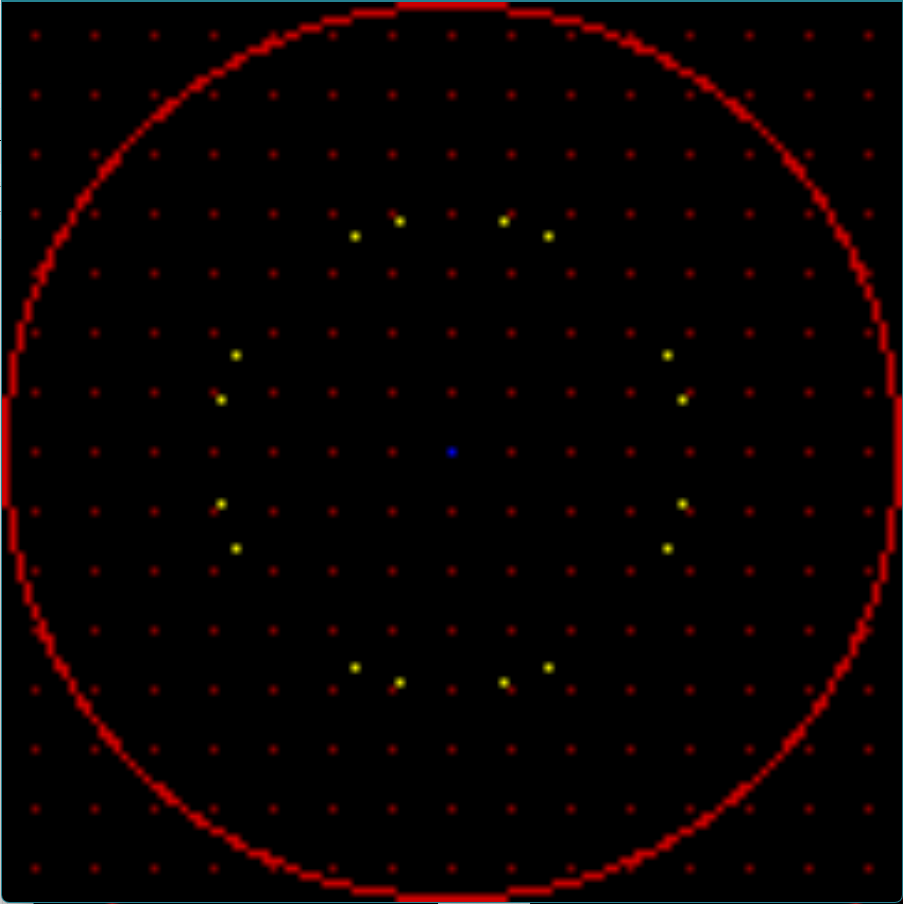
\includegraphics[width=0.7\textwidth]{wavefront.png}
\caption{
Two-dimensional cross section of the lattice wavefront at successive
iterations. The contours approach the circular isosurfaces expected
from the reconstructed Euclidean metric.
}
\label{fig:wavefront}
\end{figure}

\section{Discussion and Outlook}
\label{sec:discussion}

This model shows that Euclidean geometry can be reconstructed dynamically from local causal arithmetic. Limitations include the need for an initial source and potential anisotropy on cubic lattices during active transient propagation phases before total convergence. Future work encompasses multiple sources, non-Euclidean metrics, discrete curvature, higher dimensions, and dedicated hardware implementations (such as FPGA systolic arrays). The framework directly connects to digital physics, causal set theory, and emergent spacetime models.

\section{Conclusion}

We have introduced a local integer propagation model that exactly
reconstructs the Euclidean squared metric through purely local additive
updates. The result demonstrates that the quadratic form

\[
x^2+y^2+z^2
\]

can be recovered without multiplications, floating-point arithmetic,
or explicit global coordinate evaluation during propagation.

The method establishes a direct connection between local additive
propagation rules and exact metric reconstruction on regular lattices.

Potential applications include cellular automata, distance-field
computation, parallel hardware architectures, and discrete geometric
models.

\begin{thebibliography}{20}
\bibitem{danielsson1980} Per-Erik Danielsson. Euclidean Distance Mapping. \textit{Computer Graphics and Image Processing}, 1980.
\bibitem{sethian1996} J. A. Sethian. A Fast Marching Level Set Method for Monotonically Advancing Fronts. \textit{Proc. Natl. Acad. Sci.}, 1996.
\bibitem{dijkstra1959} Edsger W. Dijkstra. A Note on Two Problems in Connexion with Graphs. \textit{Numer. Math.}, 1959.
\bibitem{case2001lattice} J. Case, D. S. Rajan, and A. M. Shende. Lattice computers for approximating euclidean space. \textit{Journal of the ACM}, 48(1):110--144, 2001.
\bibitem{felzenszwalb2012distance} P. F. Felzenszwalb and D. P. Huttenlocher. Distance Transforms of Sampled Functions. \textit{Theory of Computing}, 2012.
\bibitem{neto2026arithmetico} A. Neto. Arithmetico: Euclidean Geometry from Unsigned Integer Arithmetic. GitHub repository, 2026.
\end{thebibliography}
\end{document}